
\documentclass{exam}

\usepackage{units} 
\usepackage{graphicx}
\usepackage[fleqn]{amsmath}
\usepackage{cancel}
\usepackage{float}
\usepackage{mdwlist}
\usepackage{booktabs}
\usepackage{cancel}
\usepackage{polynom}
\usepackage{caption}
\usepackage{fullpage}
\usepackage{xfrac}
\usepackage{enumerate}

\newcommand{\degree}{\ensuremath{^\circ}} 
\everymath{\displaystyle}

% \begin{figure}[H]
%   \centering
%   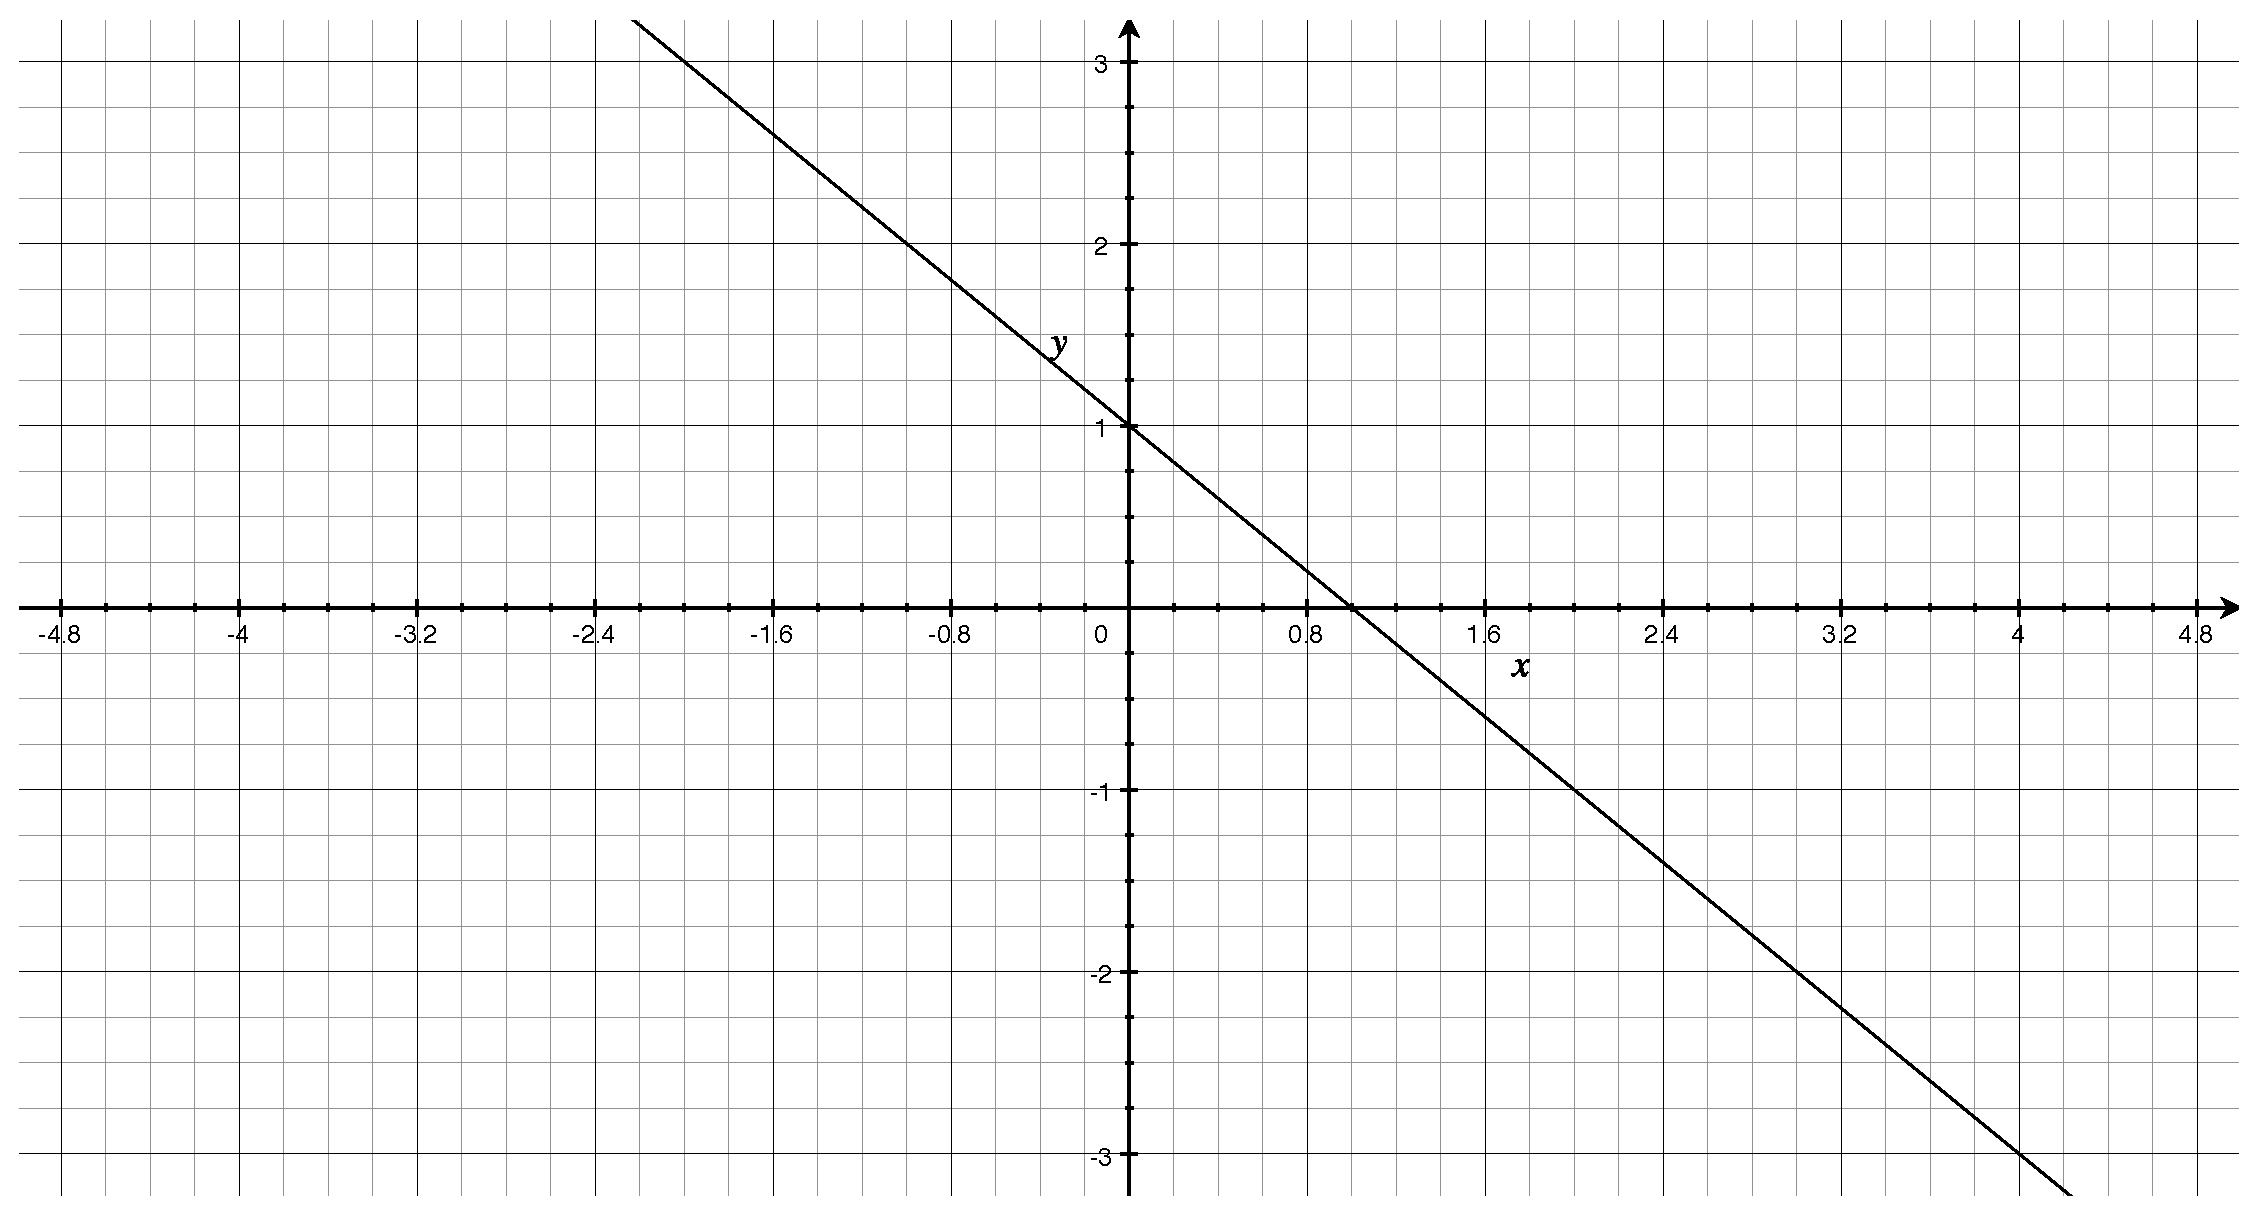
\includegraphics[scale=0.9]{problem7.eps}
%   \caption*{Problem 7}
% \end{figure}

% \begin{tabular}{cc}
%   \toprule
%   period & amplitude \\
%   \midrule
%   value one & value two
%   \bottomrule
% \end{tabular}

\printanswers

\ifprintanswers 
  \usepackage{2in1, lscape} 
\fi

\date{June 17, 2013}
\author{}
\title{Math 141 \\ Homework 15}

\begin{document}

  \maketitle

  \section{Homework}

  Section 4.3: TO DO

 \section{Extra Credit}
  Section 4.2: TO DO

  \ifprintanswers
    \begin{description}
      \item[75]
        answer here
    \end{description}
  \fi

  \section{Review}

  \begin{enumerate}

    \item $f(x) = x^3 - 1$ 

  \end{enumerate}

  \ifprintanswers
    \section{Section 4.3}

    \begin{description}

      \item[1] 
        \begin{align*}
          \log_3 \sqrt{27} &= \log_3 27^{1/2} \\
                           &= \frac{1}{2} \log_3 27 \\
                           &= \frac{3}{2} \\
        \end{align*}

      \item[2] 
        \begin{align*}
          \log_2 160 - \log_2 5 &= \log_2 \frac{160}{5} \\
                                &= \log_2 32 \\
                                &= 5 \\
        \end{align*}

      \item[3] 
        \begin{align*}
          \log 4 + \log 25 &= \log 100 \\
                           &= 2 \\
        \end{align*}

      \item[4] 
        \begin{align*}
          \log \frac{1}{\sqrt{1000}} &= \log \left( 10^3 \right)^{-1/2} \\
                                     &= - \frac{1}{2} \log 10^3 \\
                                     &= -\frac{3}{2} \\
        \end{align*}

      \item[5] 
        \begin{align*}
          \log_4 192 - \log_4 3 &= \log_4 \frac{192}{3} \\
                                &= \log_4 63 \\
                                &= 3 \\
        \end{align*}

      \item[6] 
        \begin{align*}
          \log_{12} 9 + \log_{12} 16 &= \log_{12} 144 \\
                                     &= 2 \\
        \end{align*}

      \item[7] 
        \begin{align*}
          \log_2 6 - \log_2 15 + \log_2 20 &= \log_2 \frac{6 \cdot 20}{15} \\
                                           &= \log_2 8 \\
                                           &= 3 \\
        \end{align*}

      \item[8] 
        \begin{align*}
          \log_3 100 - \log_3 18 - \log_3 50 &= \log_3 \frac{1}{9} \\
                                             &= -2 \\
        \end{align*}

      \item[9] 
        \begin{align*}
          \log_4 16^{100} &= 100 \log_4 16 \\
                          &= 200 \\
        \end{align*}

      \item[10] 
        \begin{align*}
          \log_2 8^{33} &= 33 \log_2 8 \\
                        &= 99 \\
        \end{align*}

      \item[11] 
        \begin{align*}
          \log \left( \log 10^{10,000} \right) &= \log 10,000 \\
                                               &= 4 \\
        \end{align*}

      \item[12] 
        \begin{align*}
          \ln \left( \ln e^{e^{200}} \right) &= \ln \left( e^{200} \right) \\
                                             &= 200 \\
        \end{align*}

    \end{description}

  \else
    \vspace{2 cm}
    \begin{quote}
      \begin{em}
        TO DO
      \end{em}
    \end{quote}

    \hspace{1 cm} --Carl Jung
  \fi

\end{document}

